%% LyX 1.6.4 created this file.  For more info, see http://www.lyx.org/.
%% Do not edit unless you really know what you are doing.
\documentclass[11pt,english,twocolumn]{article}
\usepackage[T1]{fontenc}
\usepackage[latin9]{inputenc}
\usepackage{array}
\usepackage{graphicx}

\makeatletter

%%%%%%%%%%%%%%%%%%%%%%%%%%%%%% LyX specific LaTeX commands.
%% Because html converters don't know tabularnewline
\providecommand{\tabularnewline}{\\}

%%%%%%%%%%%%%%%%%%%%%%%%%%%%%% User specified LaTeX commands.
%% LyX 1.6.4 created this file.  For more info, see http://www.lyx.org/.
%% Do not edit unless you really know what you are doing.



\usepackage[letterpaper]{geometry}

\geometry{verbose,tmargin=1in,bmargin=1in,lmargin=0.75in,rmargin=0.75in}

\makeatother

\usepackage{babel}

\begin{document}

\title{Edge-Based Cloud Computing as a Feasible Network Paradigm}


\author{Joe Elizondo and Samuel Palmer \\
 Department of Computer Science University of Texas at Austin\\
 Email: \{elizondo, spalmer\}@cs.utexas.edu }
\maketitle
\begin{abstract}
The term edge based cloud computing refers to a network of edge systems
that provide the services currently provided by data center clouds.
In this paper we present modifications to MRPerf, an existing tool
used to simulate MapReduce in data center clouds, that enable it to
simulate Hadoop MapReduce jobs in edge networks. Our results indicate
that the default Hadoop scheduler does not perform optimally in an
edge environment and should be replaced. We also conclude that bandwidth
is not a limiting factor in some MapReduce jobs for capacities that
are even available in some residential areas. 
\end{abstract}

\section{Introduction \label{sec:Introduction}}

Edge based cloud computing is a combination of two popular ideas,
edge computing and cloud computing. We believe that the combination
of these two ideas offers the potential for a high performance per
dollar ratio by leveraging the enormous amount of unused computational
power in idle home computer processors that have access to always-on
internet connections. Despite its potential this type of computing
paradigm is not being used and is only sparsely investigated. This
paper presents simulation results for MapReduce \cite{Dean04} jobs in an edge based cloud.
The high level of coordination and communication involved in MapReduce extends beyond the usual peer-to-peer and grid computing type of computation associated with edge computing. For our simulation
environment we investigated MRPerf, a MapReduce simulation tool built on top of
the network simulator ns-2, which was developed by researchers at
Virginia Tech and IBM Almaden Research Center. To simulate an edge
based network we modified parameters in our configuration to
better mimic a peer-to-peer type system of nodes without central infrastructure.
Each node has fewer resources and is located at a further distance
from one another than nodes in a data center. 

This paper has the following structure: Section \ref{sec:Related-Work}
discusses some related work, Section \ref{sec:Tools} presents an
overview of the tools used for our simulations, Section \ref{sec:Simulation-Design}
discusses the parameters that affect MapReduce jobs, Section \ref{sec:Implementation}
discusses our implementation of the edge based simulator, Section
\ref{sec:Simulations-and-Results} discusses the simulations and and
results, Section \ref{sec:Conclusions} presents the conclusions drawn
from the simulation results, and Section \ref{sec:Future-Research}
discusses potential future research in the area of edge based cloud
computing.


\section{Related Work\label{sec:Related-Work}}

\cite{Zaharia08} presented LATE, a scheduling algorithm to handle
heterogeneity in a data center environment. LATE attempts to schedule
tasks based on the longest approximate time to completion. The approximation
is based on the heterogeneity of the nodes and the current progress
of the task. The work presented in \cite{Zaharia08} provides useful
insights into the scheduling process in heterogeneous environments.

In general, work applying cloud computing concepts directly to edge
networks is sparse and this area of research is still in a stage of
early development. Because of this our work focused more on the feasibility
of edge based cloud computing, MapReduce in particular, from the aspect
of performance and in doing so we ignored many practical issues such
as security and privacy.


\section{Tools\label{sec:Tools}}

We leveraged two existing projects for our work. The first is MRPerf
\cite{Wang09MASCOTS,Wang09LSAP}. It was designed to simulate MapReduce
jobs when provided with a network topology for a data center. MRPerf
can measure the performance of these MapReduce jobs with a good amount
of accuracy and deliver performance information to the user. 

We considered the use of a topology generator such as GT-ITM \cite{Zegura96}
or BRITE \cite{Medina01} but decided that we would obtain more realistic
results if we used information about the actual Internet instead of
generating router topologies. We decided to use the data collected
from the Rocketfuel \cite{Spring02} project which mapped a significant
portion of the Internet. These data provided us with a realistic topology
for edge based simulations.


\subsection{MRPerf\label{sub:MRPerf}}

We chose to use MRPerf because of its impressive implementation of
MapReduce and the accuracy of its simulation results. Our research
involves testing an edge computing network with demanding highly coordinated
applications. MapReduce is a good tool for testing this because its
design requires participating machines to break up a computationally
intensive job into separate tasks, requiring complex scheduling algorithms,
process the tasks, and then merge them back together upon completion.
MRPerf was build on top of two popular packages, ns-2 \cite{Fall}
and hadoop \cite{Hadoop}. MRPerf merges MapReduce and network simulation
to achieve a seamless simulation environment. MRPerf claims to have
the ability to simulate a wide range of network topologies and also
has the ability to evaluate the performance of MapReduce operations
on that network. It was originally designed for use in a data center
type infrastructure. With that in consideration, MRPerf claims to
predict simulation performance within 5.22\% of actual measurements
for map and 12.83\% for reduce for a double rack cluster with 16 to
128 cores \cite{Wang09MASCOTS}. Although MRPerf was designed to simulate
MapReduce in multi-rack data center with many nodes per rack and high
bandwidth single hop links connecting them together it allows some
flexibility since it was built on top of the ns-2 network simulator.
This gave us the capability to simulate any topology that ns-2 supports
using MRPerf. ns-2 has already proven to be capable of simulating
a large variety of networks including networks based on grid computing
and peer to peer type topologies \cite{Kun05,Zegura96} that our network
closely resembles.


\subsection{Rocketfuel}

We wanted to run our simulation on a fairly large network to get an
accurate idea of performance when route scheduling and link latency
are taken into consideration. Rocketfuel was a project completed in
2003 at the University of Washington that mapped ISP topologies using
traceroutes from 800 different vantage points. They mapped over 50
thousand IP addresses which represented about 45 thousand routers
in 537 POPs connected by 80 thousand links. Their maps cover ISPs
in the United States, Europe, Australia, and India. They claimed that
other than the maps made by the ISPs themselves the maps produced
by Rocketfuel were the most detailed maps available in 2003. We used
the link latencies discovered by the Rocketfuel project to as input
to our simulations. This allows us to use a more accurate representation
of a real edge based network for our simulations.


\section{Simulation Design\label{sec:Simulation-Design}}

In addition to using an accurate edge topology we also needed to modify
some of the parameters used in MRPerf to simulate MapReduce tasks.
MRPerf simulates MapReduce tasks based on three classes of parameters:
cluster parameters, configuration parameters, and framework parameters.
The rest of this section is dedicated to describing these parameters
as well as modifications that could be made to improve performance
in edge networks. Section \ref{sec:Implementation} describes the
modifications that we actually made to MRPerf for our evaluations. 


\subsection{Cluster parameters }

MRPerf is designed to work with a data center using racks which consist
of many nodes that are close to each other on the network, this means
that a packet many times is just one hop away from its destination.
These racks of nodes are connected together to form a cluster. In
an edge computing network there is no concept of a centralized cluster
of computational power. Edge computing networks use PCs that are connected
to the Internet via a LAN through a router or gateway. This means
that a packet's destination is almost always several network hops
away. The racks that make up a cluster have many compute nodes each
of which have several processors whereas a PC in an edge network has
anywhere from one to four processors. Another difference in the cluster
parameters is related to node heterogeneity. A data center setup has
homogeneous nodes, whereas in an edge network nodes have a high level
of heterogeneity. The interconnect topologies also play a role in
the cluster parameters. The inter/intra-rack topology of a data center
is much less complex than the Internet.


\subsection{Configuration parameters}

Configuration parameters are related to the MapReduce jobs themselves.
They adjust settings such as data chuck size, data replication, tasks
per node, and tasks in each job. All of these settings are optimized
for a data center by default. Some of the changes we have to make
will depend upon the optimal configuration of an edge computing network.
Whether data chunk size is large or small depends upon whether an
edge computing system performs better when I/O is optimized or when
parallelism is increased. The cost of data replication is clearly
higher in an edge computing network than in a data center and .


\subsection{Framework parameters}

Framework parameters deal with data placement and scheduling algorithms.
The distance of nodes relative the machine requesting jobs needs to
be considered when partitioning data across available resources. In
a data center with many compute nodes the wrong choice of data placement
can affect performance to a degree, but is not nearly as costly as
the wrong choice when compute nodes could potentially be in a different
country. MRPerf compares three types of data locality, node-local,
rack-local, rack-remote. Our simulations use the rack-remote algorithm
in MRPerf, which was the slowest for all of the data center evaluations
\cite{Wang09MASCOTS}. The scheduling algorithm can also be optimized
for edge networks to account for node heterogeneity, bandwidth capacity,
and round trip time. As discussed above the proper balance of data
chunk size, data placement, and task scheduling are important so that
the system does not suffer huge performance losses transferring large
amounts of data over relatively slow links to a non-optimal number
of nodes.


\subsection{Limitations}

There are a couple of limitations that are inherent when working with
MRPerf that are worth discussing. These limitations are related to
disk storage and simulation of node reliability. The former works
to our advantage in this case. MRPerf only allows for one single storage
device per node. In a data center this might be an unusual constraint
however since the average PC that constitutes our edge computing network
will have only a single storage disk this should not present a problem
in our evaluation. The early release of MRPerf available does not
currently support realistic node failures or lagging nodes. Ideally,
we would have been able to simulate lagging nodes and failed nodes
in our evaluation. However, without an accurate mechanism to simulate
these cases we leave this for future work.


\section{Implementation\label{sec:Implementation}}

The goal of our implementation was to discover if the MapReduce framework
is feasible in an edge network. The implementation used in our simulations
addressed some but not all of the issues discussed in Section \ref{sec:Simulation-Design}.
We discuss the issues that have not been addressed in Section \ref{sec:Future-Research}.


\subsection{MRPerf Input and Pre-Processing Overview}

%
\begin{figure}
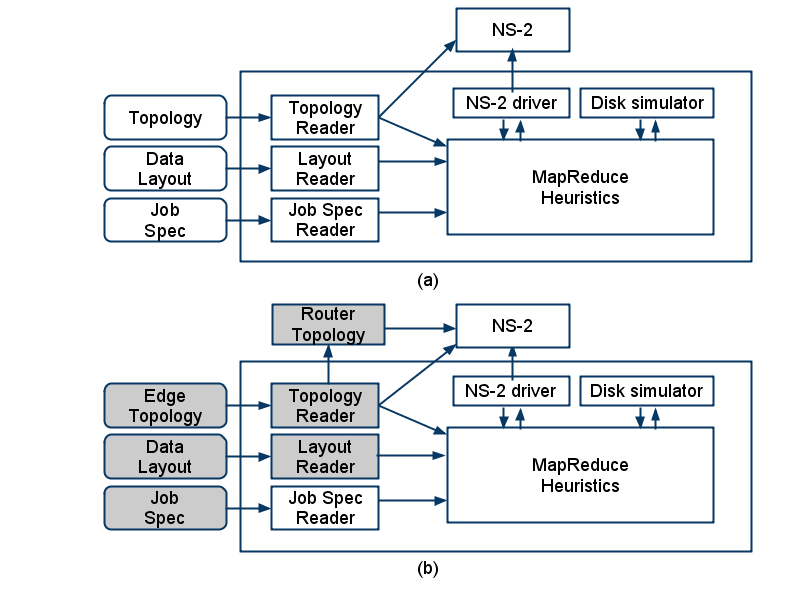
\includegraphics[width=7.8cm]{mrperf_arch}

\caption{(a) shows the original MRPerf architecture. The shaded components
in (b) were changed or added for the edge based MapReduce simulations.\label{fig:MRPerf-arch}}



\end{figure}


Figure \ref{fig:MRPerf-arch} (a) shows the original MRPerf architecute.
The topology, data layout, and job specifications are provided as
input in the form of XML and TCL code. The topology is provided in
XML format which is parsed by a Python script. This script outputs
the necessary TCL code for use in ns-2 and an XML data layout file
which is read directly by the MRPerf module integrated into ns-2.
In addition to the XML input which specifies the topology the TCL
input contains the MapReduce job specification such as the number
of map and reduce slots available for each node. These variables are
used directly by the simulator.

Figure \ref{fig:MRPerf-arch} (b) highlights the changes and additions
to the MRPerf architecture that were required to simulate the edge
based networks. The basic idea behind our modifications was to create
\textquotedbl{}racks\textquotedbl{} each containing one node. These
one node \textquotedbl{}racks\textquotedbl{} could then use the remote
rack scheduling algorithm to receive data and tasks across the network.
The following discussion outlines the modifications made to each part
of the MRPerf architecture in order to realize this idea. 

\emph{Topology and Topology Reader.} The original construction of
MRPerf accounted for the CPU speed, amount of memory, and I/O speed
but forced all nodes participating in a computation to be homogeneous.
We changed the semantics of the topology reader to allow a different
host configuration for each rack. We then employed the use of a script
to generate sets of end hosts which we attached to the routers. Table
\ref{tab:hostSpecs} summarizes the range of specifications that we
used in our evaluation. In addition to including a range of host specifications
we modified the Topology Reader to randomly choose the bandwidth of
the last hop from the Internet router to the host based on a normal
distribution. In our evaluation we set the mean of the distribution
at 16 Mbps with a standard deviation of 8 Mbps.%
\begin{table}
\begin{tabular}{|>{\centering}m{2.6cm}|>{\centering}m{5cm}|}
\hline 
CPU speed (GHz)  & 1.5, 1.6, 1.8, 2.0, 2.3, 2.4, 2.5, 3.0, 3.2\tabularnewline
\hline 
Number of CPUs & 1, 2\tabularnewline
\hline 
Number of cores per CPU & 1, 2, 4\tabularnewline
\hline 
Number of disks & 1, 2\tabularnewline
\hline 
Disk capacity (GB) & 40, 60, 80, 100, 120, 160, 180, 200, 250, 300, 400, 450, 500, 550,
600, 650, 700, 750, 800, 850, 900, 950, 1000\tabularnewline
\hline 
Disk read bandwidth (MB/s) & 250, 260, 270, 280\tabularnewline
\hline 
Disk write bandwidth (MB/s) & 60, 65, 70, 75\tabularnewline
\hline 
NIC capacity & 100Mbps, 1Gbps\tabularnewline
\hline 
Memory capacity (GB) & 0.5, 1, 2, 3, 4, 5, 6\tabularnewline
\hline
\end{tabular}

\caption{Summary of ranges used in host specification\label{tab:hostSpecs}}

\end{table}


\emph{Data Layout and Layout Reader.} The data layout components of
MRPerf control size of data chunks and the initial scheduling of data
chunks to individual disks. The semantic modification we made in the
topology portion of MRPerf forced us to also modify the initial chunk
distribution. 

\emph{Router Topology.} The original Topology Reader component of
MRPerf generated a complete data center topology script for use in
ns-2 based on a specification provided in the form of an XML document.
The results for the experiments with hosts distributed across the
mapped Internet are presented in Figure TCL code that is interpreted
by ns-2. For our simulations we directly converted the topologies
provided by the Rocketfuel results into TCL code and simply made the
Topology Reader output a call to this code. 


\section{Simulations and Results\label{sec:Simulations-and-Results}}

We conducted simulations in which we varied several aspects of the
simulation including the number of nodes, chunk size, link bandwidth,
and the number of map and reduce slots per node. The results presented
in this section are the average over five simulations with the same
parameters but different seeds for our pseudo-random number generator.
All of the hosts in the edge simulations have specifications taken
at random from the specifications presented in Table \ref{tab:hostSpecs}.
Each simulation consisted of a MapReduce job sorting one gigabyte
of data. All statistically insignificant data points have been removed.

%
\begin{figure}
\raggedright{}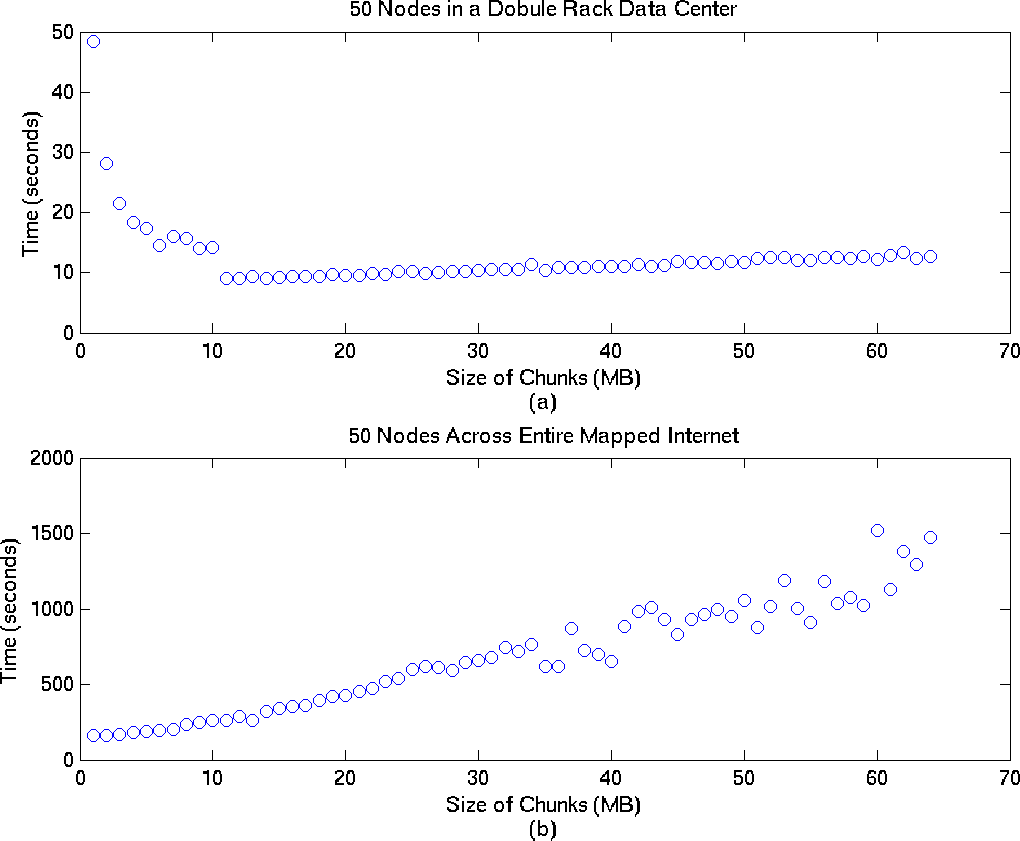
\includegraphics[width=8.7cm]{results/results_dataCenterChunkSizeBoth}\caption{Results for 50 node topologies in a double rack data center configuration
(a) and a random configuration distributed across the entire mapped
portion of the Internet (b) in which the size of the data chunks was
variable.\label{fig:chunkSize}}

\end{figure}


For the chunk size simulations we conducted two types of simulations,
one in which the nodes are in a double rack data center and one in
which nodes are randomly distributed throughout the mapped portion
of the Internet. For both types we used 50 node topologies which we
held constant for all simulations. The total MapReduce run times calculated
for these simulations are presented in Figure \ref{fig:chunkSize}.

%
\begin{figure}
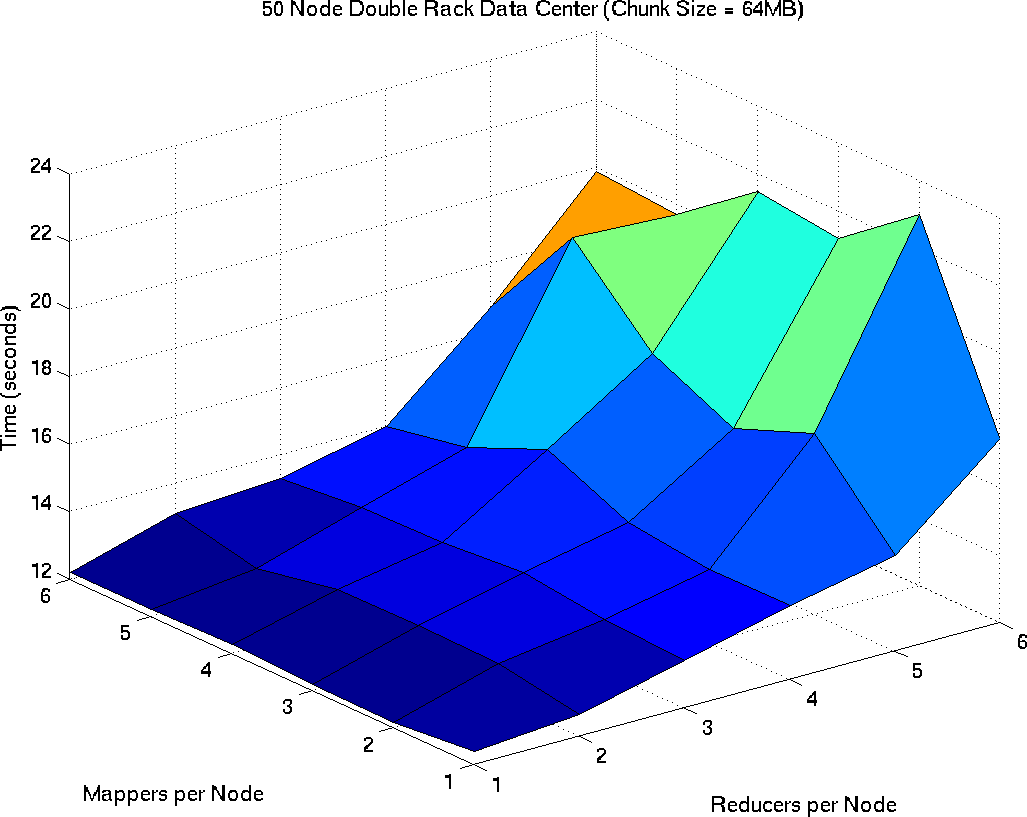
\includegraphics[width=8.7cm]{results/results_dataCenterMapperReducer_shaded}\caption{Results for 50 node double rack data center topology in which the
number of map and reduce slots available on each host was variable.\label{fig:dataCenterMapperReducer}}



\end{figure}
%
\begin{figure}
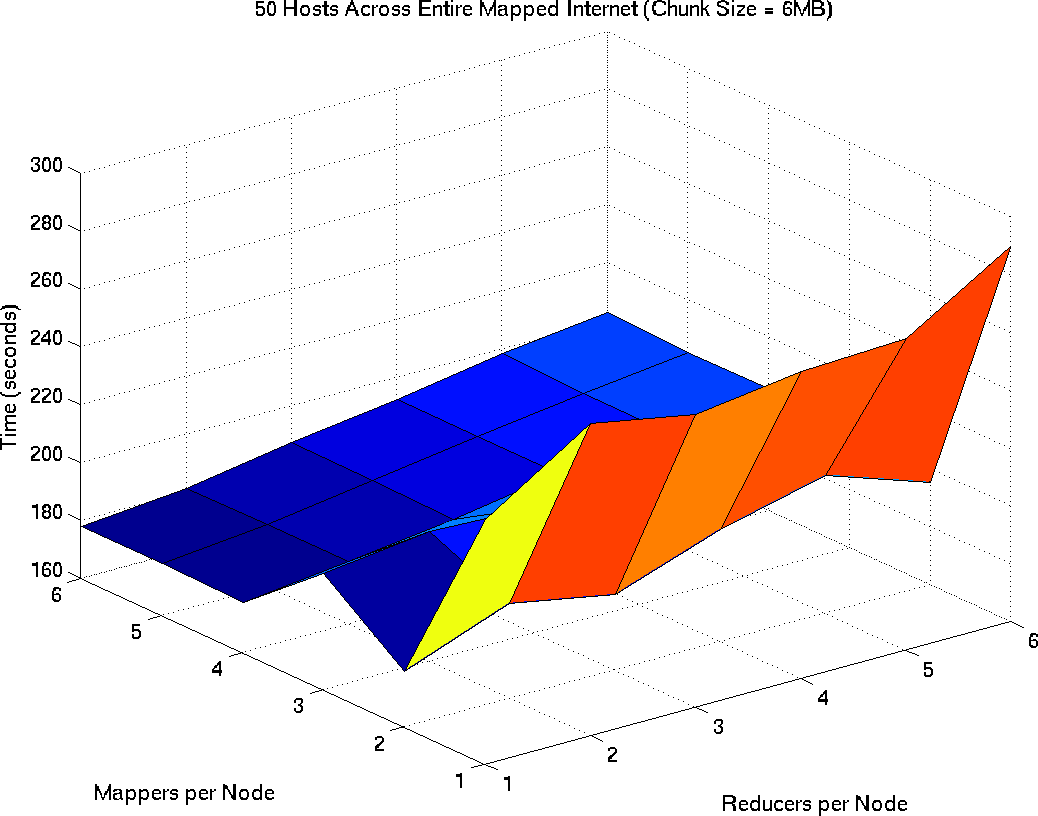
\includegraphics[width=8.7cm]{results/results_mapperReducer_shaded}

\caption{Results for a 50 node topology randomly distributed across the mapped
portion of the Internet in which the number of map and reduce slots
available on each host was variable.\label{fig:mapperReducer}}

\end{figure}


For the simulations in which we varied the number of available map
slots and the available number of reduce slots per node we used a
chunk size of 6 MB and a 50 node topology randomly distributed across
the mapped portion of the Internet. The topology was held constant
as we varied the number of available map and reduce slots per node.
The results from these simulations are presented in Figure \ref{fig:mapperReducer}.
We also ran similar simulations on a 50 node double rack data center
configuration with a 64 MB chunk size. These results are presented
in Figure \ref{fig:dataCenterMapperReducer}.

%
\begin{figure}
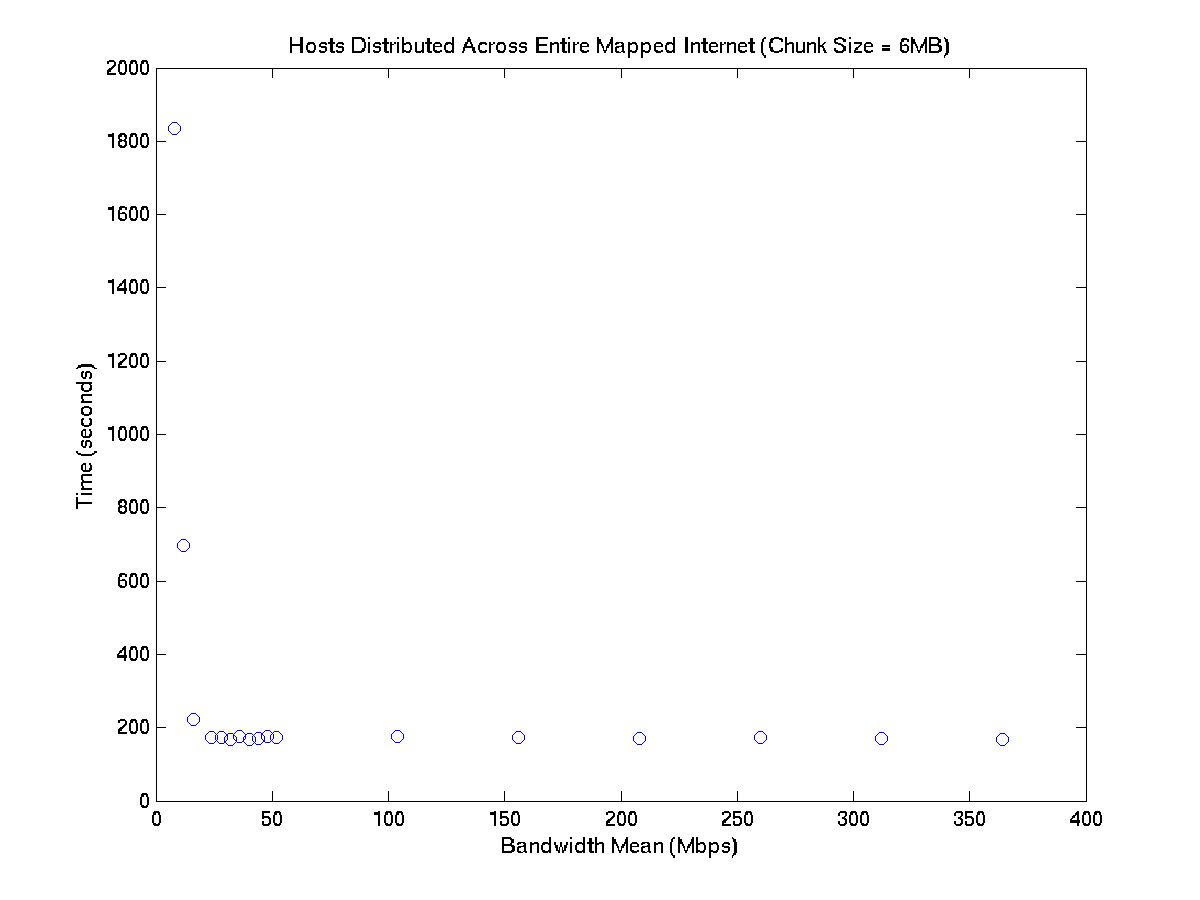
\includegraphics[width=8.7cm]{results/results_BW}\caption{Results for a 50 node topology distributed across the mapped portion
of the Internet in which the mean of the normal distribution that
we used to randomly assign the bandwidth of the link connected to
each node varies. \label{fig:bandwidth}}

\end{figure}


In the simulations in which we varied the bandwidth of the link connecting
the end hosts to the routers we used a 50 node topology where nodes
were distributed across the entire mapped Internet. This topology
was held constant as we varied the mean of the normal distribution
that was used to assign the bandwidth of the end hosts' links. The
standard deviation of the normal distribution was held at 8Mbps. The
results from these simulations are presented in Figure \ref{fig:bandwidth}.

%
\begin{figure}
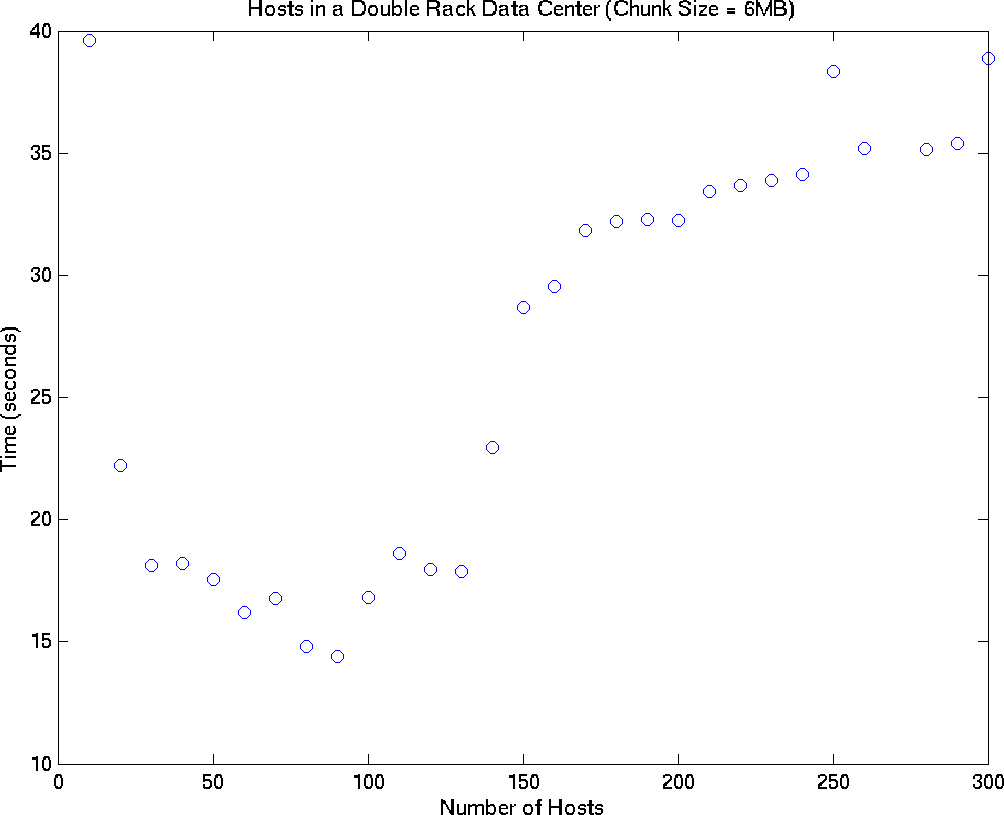
\includegraphics[width=8.7cm]{results/results_dataCenterNumHosts}\caption{Results for double rack data center topologies in which the total
number of nodes was variable.\label{fig:dataCenterNumHosts}}

\end{figure}
%
\begin{figure}
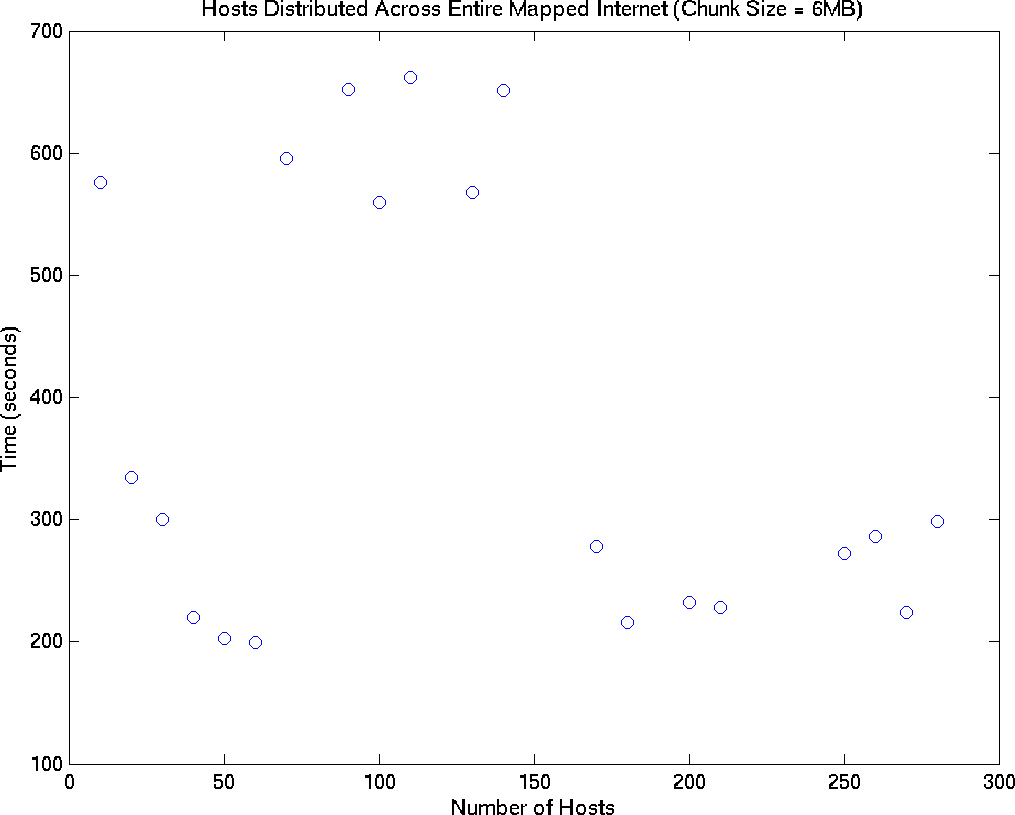
\includegraphics[width=8.7cm]{results/results_numHosts}

\caption{Results for topologies in which each consecutive point represents
the running time when 10 additional hosts are randomly added to the
previous topology. Hosts are distributed across the entire mapped
portion of the Internet.\label{fig:numHosts}}

\end{figure}
%
\begin{figure}
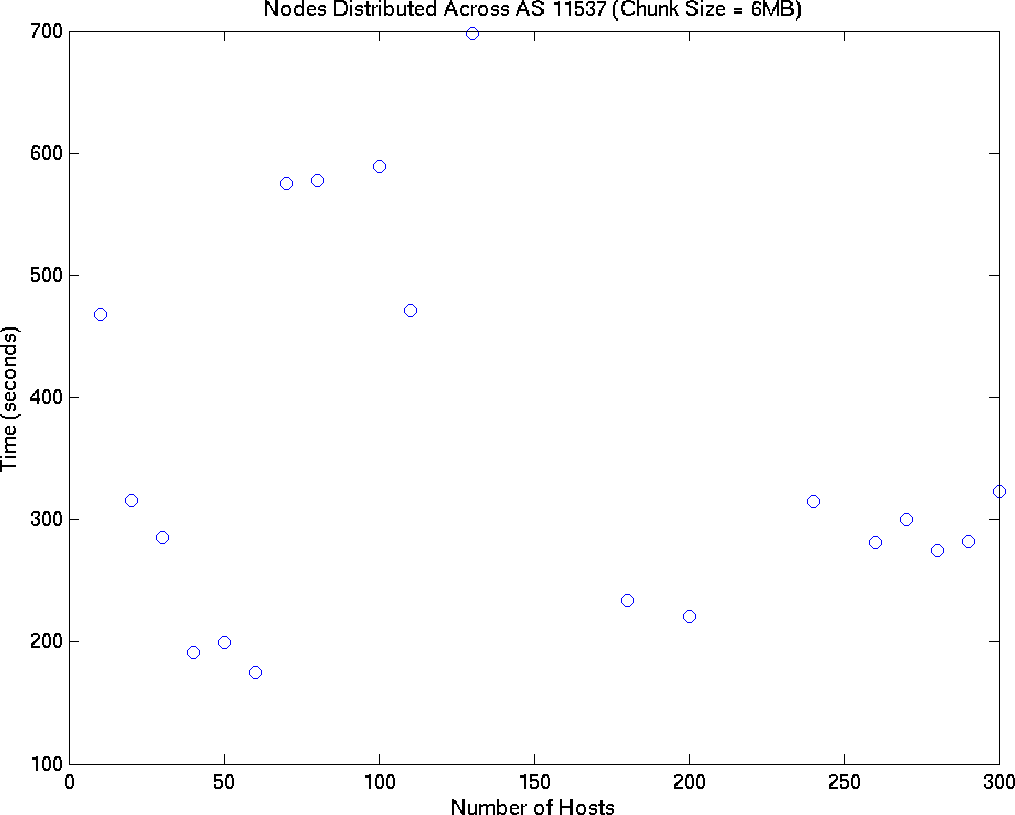
\includegraphics[width=8.7cm]{results/results_numHosts_oneAS}

\caption{Results for topologies in which each consecutive point represents
the running time when 10 additional hosts are randomly added to the
previous topology. Hosts are distributed across AS 11537 which spans
the entire United States and parts of southern Canada.\label{fig:numHosts_oneAS}}

\end{figure}


We ran three types of simulations that varied the number of nodes.
We varied the number of nodes in a double rack data center, distributed
across the mapped portion of the Internet, and distributed across
one autonomous system consisting of 15 mapped routers which span the
United States. Each consecutive simulation for the edge based data
kept the previous simulation's topology and added 10 additional nodes
randomly distributed throughout the topology. The results for the
data center and edge based simulations are presented in Figures \ref{fig:dataCenterNumHosts},
\ref{fig:numHosts}, and \ref{fig:numHosts_oneAS}.


\section{Conclusions\label{sec:Conclusions}}

From our results we can conclude that the data chunk size used in
edge based MapReduce jobs should be considerably smaller than what
is usually used in data center MapReduce jobs. Figure \ref{fig:chunkSize}
shows that while certain data center topologies can suffer if the
chunk size is too small the edge based network produces the best results
when the chunk size is small. 

The results presented in \ref{fig:mapperReducer} shows that edge-based
MapReduce jobs benefit when the number of available map slots on each
node increases but does not necessarily benefit as the number of reduce
slots available on each node increases. Figure \ref{fig:dataCenterMapperReducer}
indicates that increasing the number of map slots available on each
node does not affect the performance in the double rack data center
topology but increasing the number of reduce slots available has a
negative impact on the performance. This suggests that the number
of map slots and reduce slots should be configured carefully not only
to suit the type of MapReduce job that is running but also based on
the configuration of the topology. 

We can conclude from Figure \ref{fig:bandwidth} that adding additional
bandwidth to the end host links is no longer beneficial to the MapReduce
job performance after a certain bandwidth is reached. For the topology
used in the simulation this point is at about 20 Mbps. This suggests
that bandwidth could be a limiting factor for the other simulations
that we ran which used a mean host link bandwidth of 16 Mbps. 

We can see from Figure \ref{fig:dataCenterNumHosts} that the total
run time increases as more nodes are added after a certain point for
the data center topology evaluated. This is probably caused because
the sort algorithm becomes I/O bound and no longer benefits from extra
computational power. It is more difficult to draw conclusions about
the effects of adding more nodes in an edge based cloud. Perhaps the
only definite conclusion that we can draw is that the default scheduler
should be replaced by one that is aware of the network topology and
node specifications. In our evaluation it was possible for the scheduler
to do very well with one topology and very poorly when a distant node
is added which the scheduler blindly scheduled tasks to. The development
of this new scheduler is left for future work.


\section{Future Research\label{sec:Future-Research}}

We did not present results related to modifications to the Hadoop
scheduling algorithm used by MRPerf. This is primarily because the
early release of MRPerf we used for our simulations does not support
realistic node failures. We are confident that a scheduling algorithm
that is aware of the round trip times to each node and heterogeneity
of the nodes would perform better than the default Hadoop scheduling
algorithm. An analysis that involves the simulation of node churn
is also left for future work. 

A possible alternate simulation tool to MRPerf is CloudSim \cite{Buyya09}.
Future research could investigate the use of MapReduce with this Java
based simulation tool that has recently been developed. CloudSim was
built on top of the existing tools, JavaSim and GridSim, which have
already proven themselves valid for simulation. CloudSim itself is
an effort to add a new layer of features on top of these tools that
are more critical and immediately relevant to cloud computing. By
abstracting away all the lower levels CloudSim can focus on doing
its job correctly and at the same time trust that the layers below
are functioning correctly as well. The results gathered from simulation
with this tool would be a valuable comparison to the results we present
in this paper. Other avenues for research could address the security
and privacy implications for this type of computing paradigm.

\bibliographystyle{acm} \nocite{*} \bibliographystyle{plain}
\nocite{*}
\bibliography{finalreport}

\end{document}
